Using the sample Java web application %
MyBatis JPetStore,\footnote{\url{http://www.mybatis.org/spring/sample.html}} this example %
demonstrates how to employ \KiekerMonitoringPart{} for monitoring a Java application %
running in a Java~EE container---in this case Jetty.\footnote{\url{http://www.eclipse.org/jetty/}} %
Monitoring probes based on the Java~EE Servlet API, Spring, %
and AspectJ are used to monitor execution, trace, and session data (see Section~\ref{chap:aspectJ}). %
The directory \dir{\JavaEEServletExampleDistro/} contains the prepared Jetty %
server with the MyBatis JPetStore application and the \Kieker-based demo %
analysis application known from \url{http://demo.kieker-monitoring.net/}. %

\section{Setting}

The subdirectory \file{jetty-hightide-jpetstore/} includes the %
Jetty server with the JPetStore application already deployed to the server's %
\file{webapps/} directory. The example is prepared to use two alternative %
types of \Kieker{} probes: either the \Kieker{} Spring interceptor (default) or the 
\Kieker{} AspectJ aspects. Both alternatives additionally use \Kieker{}'s Servlet 
filter. %

\paragraph{Required Libraries and \KiekerMonitoringPart{} Configuration}

Both settings require the files \file{\aspectJWeaverJar{}} and \file{\mainJar}, %
which are already included in the webapps's \dir{WEB-INF/lib/} directory. %
Also, a \Kieker{} configuration file is already included in the Jetty's root directory, %
where it is considered for configuration by \KiekerMonitoringPart{} in both modes. 

\paragraph{Servlet Filter (Default)}

The file \file{web.xml} is located in the webapps's %
\dir{WEB-INF/} directory. \Kieker{}'s Servlet filters are already enabled: 

\setXMLListing
\lstinputlisting[firstline=50,lastline=61, numbers=none, linewidth=1\textwidth, caption=Enabling the Servlet filter in \file{web.xml}]{\JavaEEServletExampleDir/jetty-hightide-jpetstore/webapps/jpetstore/WEB-INF/web.xml}

\noindent This filter can be used with both the Spring-based and the %
AspectJ-based instrumentation mode.

\paragraph{Spring-based Instrumentation (Default)}

\Kieker{}'s Spring interceptor are already enabled in the file 
\file{applicationContext.xml}, located in the webapps's \dir{WEB-INF/} directory: 

\setXMLListing
\lstinputlisting[firstline=38,lastline=43, numbers=none, linewidth=1\textwidth, caption=Enabling the Spring interceptor in \file{applicationContext.xml}]{\JavaEEServletExampleDir/jetty-hightide-jpetstore/webapps/jpetstore/WEB-INF/applicationContext.xml}

\NOTIFYBOX{When using, for example, the \texttt{@Autowired} feature in your Spring beans, it can be necessary to force the usage of CGLIB proxy objects with \texttt{<aop:aspectj-autoproxy proxy-target-class="true"/>}.}

\paragraph{AspectJ-based Instrumentation}

\enlargethispage{1cm}

In order to use AspectJ-based instrumentation, the following changes need to 
be performed. The file \file{start.ini}, located in Jetty's root directory, %
allows to pass various JVM arguments, JVM system properties, and other options %
to the server on startup. When using AspectJ for instrumentation, the respective %
JVM argument needs to be activated in this file: %

\setPropertiesListing
\lstinputlisting[firstline=32,lastline=35, linewidth=1\textwidth,caption=Enabling the AspectJ weaver in Jetty's \file{start.ini}]{\JavaEEServletExampleDir/jetty-hightide-jpetstore/start.KiekerAspectJActivated.ini}

\noindent The AspectJ configuration file \file{aop.xml} is already located in the %
webapps's\linebreak \dir{WEB-INF/classes/META-INF/} directory and configured to instrument %
the JPetStore classes with \Kieker{}'s \class{OperationExecutionAspectFull} aspect %
(Section~\ref{chap:aspectJ}). 

\

When using the AspectJ-based instrumentation, make sure to disable the Spring %
interceptor in the file \file{applicationContext.xml}, mentioned above. %

\begin{compactenum}
\item Start the Jetty server using the \file{start.jar} file. You should make %
   sure that the server started properly by taking a look at %
   the console output that appears during server startup.  
\item Now, you can access the JPetStore application by opening the URL
   \url{http://localhost:8080/jpetstore/} (Figure~\ref{fig:jpetstore}). %
   \Kieker{} initialization messages should appear in the console output. %
   
\begin{figure}[h]\centering
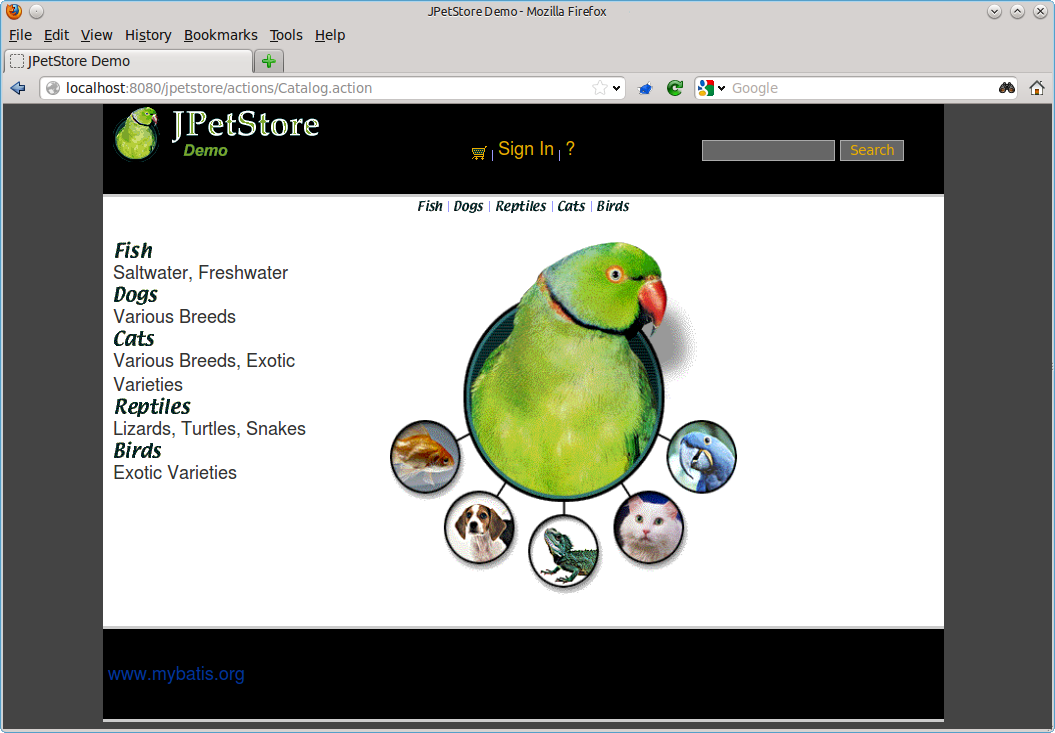
\includegraphics[width=0.8\textwidth]{images/jpetstore-example-FFscrsh}
\caption{MyBatis JPetStore}\label{fig:jpetstore}%
\end{figure}
   
\item   Browse through the application to generate some monitoring data. %
\item In this example, \Kieker{} is configured to write the monitoring data %
      to JMX in order to communicate with the \Kieker-based demo analysis %
      application, which is accessible via \url{localhost:8080/demo/}.
   
\item In order to write the monitoring data to the file system, the %
      JMX writer needs to be disabled in the file \file{kieker.monitoring.properties}, %
      which is located in the directory \file{webapps/jpetstore/WEB-INF/classes/META-INF/}.
      After a restart of the Jetty server, the Kieker startup output includes the %
      information where the monitoring data is written to (should be a %
      \dir{kieker-<DATE-TIME>/} directory) located in the default temporary %
      directory. %
   This data can be analyzed and visualized using \KiekerTraceAnalysis{}, %
   as described in Chapter~\ref{chap:aspectJ}.
\end{compactenum}

\medskip

 